\section{Random Forest}
The last classifier used in this project is the \class{RandomForestClassifier()} from \code{sklearn.ensemble}.
A random forest is a type of ensemble learning method.
An ensemble method is a machine learning technique that combines the predictions of multiple models to make more accurate predictions than any individual model.
In a random forest, a set of decision trees are typically trained on a subset of the original dataset.
The predicted class of an input sample is a vote by the trees in the forest, weighted by their probability estimates.
That is, the predicted class is the one with highest mean probability estimate across the trees.
Therefore, a random forest is not as prone to overfitting as a single decision tree, since this voting process helps to reduce the variance of the model, and the trees are trained on different parts of the dataset.

\begin{figure}[H]
    \centering
    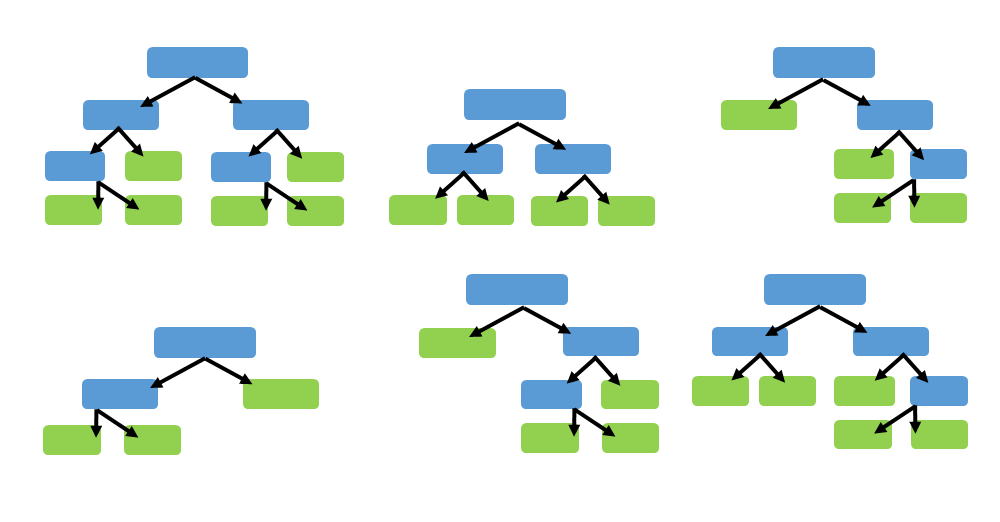
\includegraphics[scale=0.3]{figures_for_report/random_forest_simple_example}
    \captionsetup{justification=centering,margin=2cm}
    \caption{A Random Forest Illustration}\label{fig:figure}
\end{figure}


\subsection{Hyperparameters}\label{subsec:hyperparameters}
The hyperparameters were chosen similarly to the \class{DecisionTreeClassifier()} with a grid search.
The parameter grid used was the following:\\

\begin{center}
    \begin{minipage}{4in}
\begin{itemize}
    \item \code{max_depth}: [None, 10, 15, 20, 21, 22, 23]
    \item \code{min_samples_split}: [2, 4, 8]
    \item \code{criterion}: ['gini', 'entropy'] \\
\end{itemize}
            \end{minipage}
\end{center}

Which gave the best combination as:\\

\begin{tcolorbox}[colback=white,
                  arc=0pt,
                outer=0pt]
\centering \code{max_depth=21} \, \, \code{min_samples_split=4} \, \, \code{criterion=gini} \, \, \\
   \end{tcolorbox}


These values were selected due to their ability to effectively prevent overfitting and improve the accuracy of the model, just like the decision tree parameters.
Then an instance of the \class{RandomForestClassifier()} was trained, with the parameters, while keeping all others at their default values. This means that the \code{n_estimators=100}.
Additionally \code{random_state=42} was again used, and will lead to the reproduction of the results reported in the next section.

\subsection{Results}\label{subsec:results}
\begin{table}[!ht]
\begin{subtable}[c]{0.4\textwidth}
\footnotesize
\centering
\begin{tabular}{ c | c }
 \toprule
 Evaluation Metric & Accuracy Score  \\
 \midrule
 Training Accuracy &  99.79\% \\
 Test Accuracy & 84.88\% \\
 \bottomrule
\end{tabular}
\captionsetup{justification=centering,margin=1cm}
\end{subtable}
\begin{subtable}[c]{0.6\textwidth}
\footnotesize
\centering
\begin{tabular}{c | c c r}
Class & Precision & Recall & F1-Score\\
\midrule
T-shirt/Top   &    0.81  &    0.85  &    0.82 \\
Trousers   &    0.99  &    0.95  &    0.97 \\
Pullover   &    0.82  &    0.89  &    0.85\\
Dress   &    0.89  &    0.93  &    0.91\\
Shirt   &    0.73  &    0.63  &    0.68\\
\end{tabular}
\captionsetup{justification=centering,margin=1cm}
\end{subtable}
\caption{Random Forest Performance}
\label{tab:random_forest_evaluation}
\end{table}\\

The \class{RandomForest()} achieved a test accuracy of $84.88\%$ and training accuracy of $99.97\%$.
Again, the random forest classifier performs very well at correctly classifying Trouser and Dresses with a f1-score of 0.97 and 0.91 as seen in \textbf{Table 4}.
The classifier struggles with the Shirt class which achieved a f1-score of 0.69.
